\documentclass[psamsfonts]{amsart}

%-------Packages---------
\usepackage{amssymb,amsfonts}
\usepackage{semantic}
\usepackage{fullpage}
\usepackage{tikz-cd}
\usepackage{todonotes}
\usepackage{physics}
\usepackage[all,arc]{xy}
\usepackage{enumerate}
\usepackage{enumitem}
\usepackage{mathrsfs}
\usepackage{theoremref}
\usepackage{graphicx}
\usepackage[bookmarks]{hyperref}

%--------Theorem Environments--------
%theoremstyle{plain} --- default
\newtheorem{thm}{Theorem}[section]
\newtheorem{cor}[thm]{Corollary}
\newtheorem{prop}[thm]{Proposition}
\newtheorem{lem}[thm]{Lemma}
\newtheorem{conj}[thm]{Conjecture}
\newtheorem{quest}[thm]{Question}

\theoremstyle{definition}
\newtheorem{defn}[thm]{Definition}
\newtheorem{defns}[thm]{Definitions}
\newtheorem{con}[thm]{Construction}
\newtheorem{exmp}[thm]{Example}
\newtheorem{exmps}[thm]{Examples}
\newtheorem{notn}[thm]{Notation}
\newtheorem{notns}[thm]{Notations}
\newtheorem{addm}[thm]{Addendum}
\newtheorem{exer}[thm]{Exercise}
\newtheorem{innercustomexer}{Exercise}
\newenvironment{customexer}[1]
  {\renewcommand\theinnercustomexer{#1}\innercustomexer}
  {\endinnercustomexer}

\newtheorem{innercustomprob}{Problem}
\newenvironment{customprob}[1]
  {\renewcommand\theinnercustomprob{#1}\innercustomprob}
  {\endinnercustomprob}

\newtheorem{innercustomthm}{Proposition}
\newenvironment{customthm}[1]
  {\renewcommand\theinnercustomthm{#1}\innercustomthm}
  {\endinnercustomthm}

\theoremstyle{rem}
\newtheorem*{rem}{Remark}
\newtheorem{rems}[thm]{Remarks}
\newtheorem{warn}[thm]{Warning}
\newtheorem{sch}[thm]{Scholium}

\DeclareMathOperator{\Hom}{Hom}
\DeclareMathOperator{\Id}{Id}
\DeclareMathOperator{\End}{End}
\DeclareMathOperator{\ord}{ord}
\DeclareMathOperator{\Aut}{Aut}
\DeclareMathOperator{\Gal}{Gal}
\DeclareMathOperator{\RP}{\mathbb{R}\mathbb{P}}
\DeclareMathOperator{\CP}{\mathbb{C}\mathbb{P}}
\DeclareMathOperator{\Int}{Int}
\DeclareMathOperator{\bd}{bd}
\DeclareMathOperator{\supp}{supp}
\DeclareMathOperator{\sgn}{sgn}
\DeclareMathOperator{\PD}{PD}

\makeatletter
\let\c@equation\c@thm
\makeatother
\numberwithin{equation}{section}

\bibliographystyle{plain}

\begin{document}

\title{Algebraic Topology II Lecture Notes}
\author{Hidenori Shinohara}

\maketitle
\tableofcontents

\section{Geometric Description of Cocycles}

\begin{exmp}
  Let $X$ be a $\Delta$-complex and $\phi \in C^k(X; \mathbb{Z})$.
  What does it mean that $\delta \phi = 0$?
  As a toy model, we will consider a surface.
  One way to construct such a $\phi \in C^1(X; \mathbb{Z})$ is to take an oriented closed curve $\gamma$ transverse to 1-simplices.
  Then we define $\phi(\sigma)$ to be the number of intersections between $\sigma$ and $\gamma$ with signs.
  See the following example:

  \begin{figure}[!htb]
    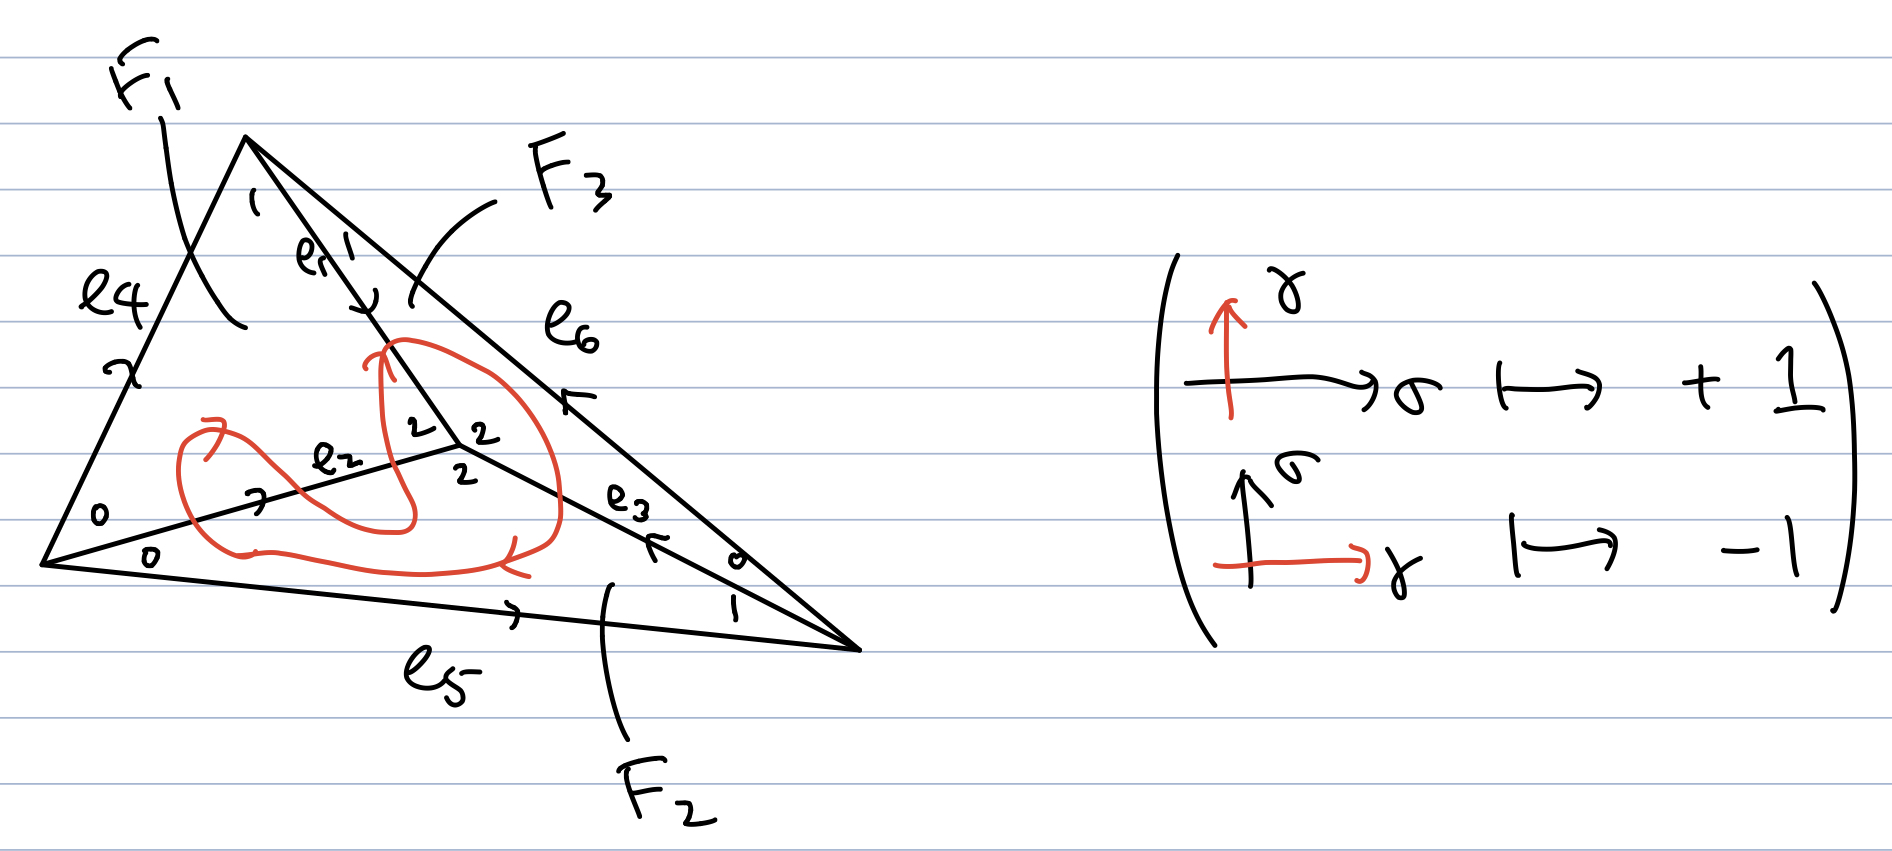
\includegraphics[width=.7\linewidth]{img/geometric_description_cocycle.jpeg}
    \caption{Oriented closed curve in a surface}
    \label{fig:cocycle}
  \end{figure}

  $\gamma$ gives us the following 1-cocycle $\phi$ which maps each $e_i$ to an integer as following:
  \begin{align*}
    & e_1 \mapsto 1 \\
    & e_2 \mapsto 1 - 1 + 1 = 1 \\
    & e_3 \mapsto 1 \\
    & e_4 \mapsto 0 \\
    & e_5 \mapsto 0 \\
    & e_6 \mapsto 0.
  \end{align*}

  Then $\delta\phi = 0$ because
  \begin{align*}
    (\delta\phi)(F_1) &= \phi(\partial F_1) = \phi(e_1) - \phi(e_2) + \phi(e_4) = 0 \\
    (\delta\phi)(F_2) &= \phi(\partial F_2) = \phi(e_3) - \phi(e_2) + \phi(e_5) = 0 \\
    (\delta\phi)(F_3) &= \phi(\partial F_3) = \phi(e_1) - \phi(e_3) + \phi(e_6) = 0.
  \end{align*}

  This is not a coincidence because $\phi(\partial\sigma)$ represents 
  \begin{center}
    (the number of times $\gamma$ enters $\sigma$) - (the number of times $\gamma$ exists $\sigma$)
  \end{center}
  which is always 0 for any 2-simplex $\sigma$ and any traverse closed oriented curve $\gamma$.
  In this case, we call $\phi$ the \textbf{Poincare dual} to $\gamma$, or simply $\phi = \PD(\gamma)$, and this concept can be generalized further.
\end{exmp}

\begin{defn}
  Let $X$ be a topological manifold of dimension $n$.
  Let $\gamma$ be an $(n - k)$-cycle in $X$ transverse to the $k$-skeleton of $X$.
  Define $\phi \in C^{k}(X; \mathbb{Z})$ such that
  \begin{align*}
    \phi(\sigma) &= \text{The number of intersections between $\sigma$ and $\gamma$ with signs}.
  \end{align*}
  Then we call $\phi$ the \textbf{Poincare dual} of $\gamma$ and denote it by $\phi = \PD(\gamma)$.
\end{defn}

\begin{exmp}
  We will look at a torus which is a slightly more complicated example.
  \begin{figure}[!htb]
    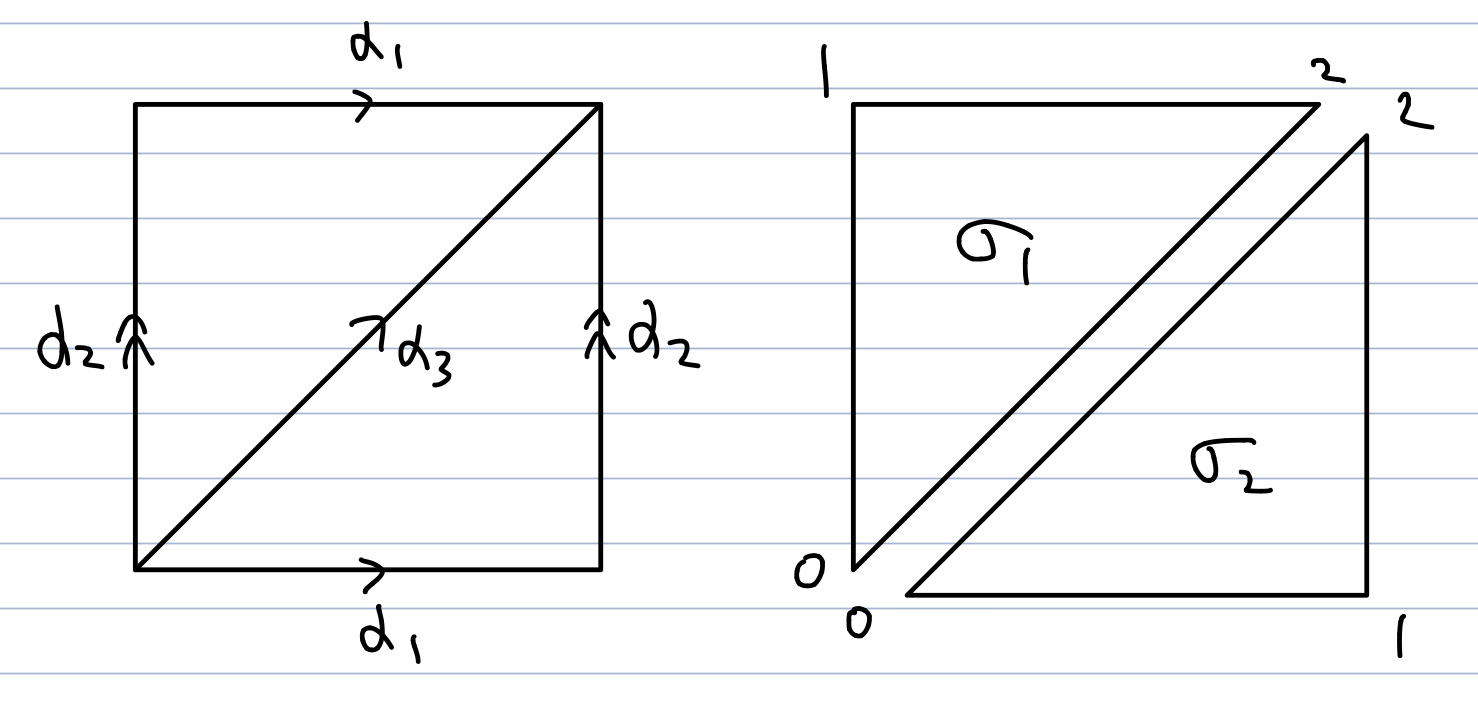
\includegraphics[width=.5\linewidth]{img/torus.jpeg}
    \caption{Torus}
    \label{fig:torus}
  \end{figure}
  We obtain the following cellular chain complex from Figure \ref{fig:torus}:
  \begin{center}
    \begin{tikzcd}[cells={nodes={minimum height=2em}}]
      C_2 = \ev{\sigma_1, \sigma_2} \arrow[r] & C_1 = \ev{\alpha_1, \alpha_2, \alpha_3} \arrow[r] & C_0 = \ev{v} \\
      \sigma_i \arrow[r, maps to]             & \alpha_1 + \alpha_2 - \alpha_3                    & \\
                                              & \alpha_i \arrow[r, maps to]                       &  0 \\
    \end{tikzcd}
  \end{center}
  Thus
  \begin{align*}
    H_i(T^2) &= \begin{cases}
      \mathbb{Z}   & (i = 0, 2) \\
      \mathbb{Z}^2 & (i = 1).
    \end{cases}
  \end{align*}
  Now, we will examine the cellular cochain complex.
  \begin{align*}
    \delta(v^{\ast})(\alpha_i)
      &= v^{\ast}(\partial \alpha_i) \\
      &= v^{\ast}(0) \\
      &= 0
  \end{align*}
  for any $\alpha_i \in C_1$.
  Therefore, $\delta(v^{\ast}) = 0$.
  \begin{align*}
    \delta(\alpha_1^{\ast})(\sigma_i)
      &= \alpha_1^{\ast}(\partial(\sigma_i)) \\
      &= \alpha_1^{\ast}(\alpha_1 + \alpha_2 - \alpha_3) \\
      &= 1
  \end{align*}
  for any $\sigma_i \in C_2$.
  By performing similar calculation on $\alpha_2^{\ast}$ and $\alpha_3^{\ast}$, we obtain
  \begin{center}
    \begin{tikzcd}[cells={nodes={minimum height=2em}}]
      C^2 = \ev{\sigma_1^{\ast}, \sigma_2^{\ast}} & C^1 = \ev{\alpha_1^{\ast}, \alpha_2^{\ast}, \alpha_3^{\ast}} \arrow[l] & C^0 = \ev{v^{\ast}} \arrow[l] \\
      \sigma_1^{\ast} + \sigma_2^{\ast}           & \alpha_1^{\ast}, \alpha_2^{\ast} \arrow[l, maps to]                    & \\
      -(\sigma_1^{\ast} + \sigma_2^{\ast})        & \alpha_3^{\ast} \arrow[l, maps to]                                     & \\
                                                  & 0                                                                      & v^{\ast} \arrow[l, maps to] \\
    \end{tikzcd}
  \end{center}
  Thus
  \begin{align*}
    H^i(T^2) &= \begin{cases}
      \mathbb{Z}   & (i = 0, 2) \\
      \mathbb{Z}^2 & (i = 1).
    \end{cases}
  \end{align*}

  \begin{itemize}
    \item
      $H^0(T^2) = \ev{v^{\ast}} / 0$, so $H^0(T^2)$ is generated by $[v^{\ast}]$.
    \item
      $H^2(T^2)$ is generated by $[\sigma_2^{\ast}]$ because $H^2(T^2) = \ev{\sigma_1^{\ast}, \sigma_2^{\ast}} / \ev{\sigma_1^{\ast} + \sigma_2^{\ast}}$.
  \end{itemize}
  We can picture $H^1(T^2)$ by using Poincare duals.
  \begin{figure}[!htb]
    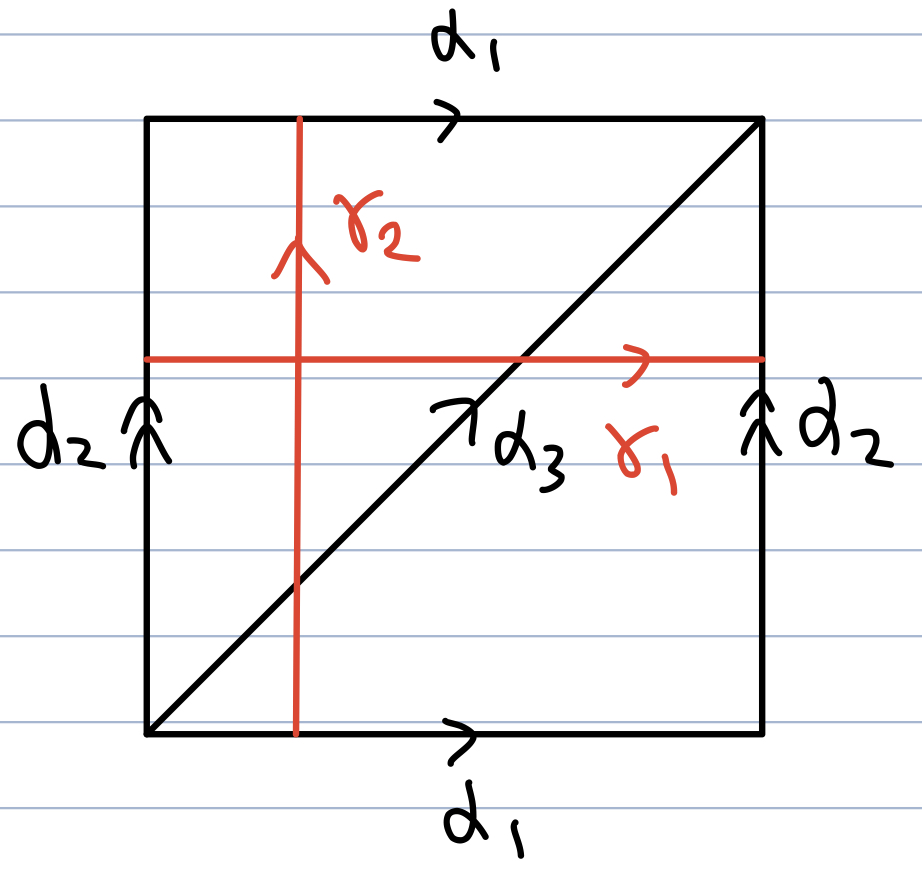
\includegraphics[width=.5\linewidth]{img/torus_pd.jpeg}
    \caption{Torus Poincare Duals}
    \label{fig:torus_pds}
  \end{figure}
  Let $\phi_1 = \PD(\gamma_1), \phi_2 = \PD(\gamma_2)$.
  Then $\phi_1(\alpha_1) = 0, \phi_1(\alpha_2) = 1, \phi_1(\alpha_3) = 1$, and $\phi_2(\alpha_1) = -1, \phi_2(\alpha_2) = 0, \phi_2(\alpha_3) = -1$.
  Moreover,
  \begin{align*}
    (\delta\phi_1)(\sigma_i) &= \phi_1(\partial\sigma_i) = \phi_1(\alpha_1 + \alpha_2 - \alpha_3) = \phi_1(\alpha_1) + \phi_1(\alpha_2) - \phi_1(\alpha_3) = 0. \\
    (\delta\phi_2)(\sigma_i) &= \phi_2(\partial\sigma_i) = \phi_2(\alpha_1 + \alpha_2 - \alpha_3) = \phi_1(\alpha_1) + \phi_1(\alpha_2) - \phi_1(\alpha_3) = 0.
  \end{align*}
  Therefore, the classes represented by $\phi_1, \phi_2$ are in $H^1(T^2; \mathbb{Z})$.
  Moreover, they clearly generate $H^1(T^2; \mathbb{Z})$, so every element in $H^1(T^2; \mathbb{Z})$ can be considered as a function with a fixed closed curve that counts the number of times the curve intersects a given 1-simplex.

  Now, we will examine the cup product structure.
  By definition, we know that $[\phi_1] \smile [\phi_2] \in H^2(T^2; \mathbb{Z})$.
  Therefore, we will check what $\sigma_1, \sigma_2$ get sent to.
  \begin{align*}
    (\phi_1 \smile \phi_2)(\sigma_1)
      &= \phi_1(\sigma_1\vert_{[0, 1]})\phi_2(\sigma_1\vert_{[1, 2]}) \\
      &= \phi_1(\alpha_2)\phi_2(\alpha_1) \\
      &= -1 \cdot 1 = -1. \\
    (\phi_1 \smile \phi_2)(\sigma_2)
      &= \phi_1(\sigma_2\vert_{[0, 1]})\phi_2(\sigma_2\vert_{[1, 2]}) \\
      &= \phi_1(\alpha_1)\phi_2(\alpha_2) \\
      &= 0.
  \end{align*}
  Recall that $[\sigma_1^{\ast} + \sigma_2^{\ast}] = 0$ because $\sigma_1^{\ast} + \sigma_2^{\ast}$ is in the kernel.
  Therefore, $[\phi_1 \smile \phi_2] = [-\sigma_1^{\ast}] = [\sigma_2^{\ast}]$.
  Similarly, we obtain $(\phi_2 \smile \phi_1)(\sigma_1) = 0$ and $(\phi_2 \smile \phi_1)(\sigma_2) = -1$.
  Thus $[\phi_2 \smile \phi_1] = -[\sigma_2^{\ast}]$.

  \todo[inline,caption={}]{
    I don't understand the alternative approach using the universal coefficient theorem.
  }

  Finally, we obtain the following multiplication table for $H^{\ast}(T^2; \mathbb{Z}) \cong \mathbb{Z}\ev{1, [\phi_1], [\phi_2], [\sigma_2^{\ast}]}$:
  \begin{center}
    \begin{tabular}{| l || l | l | l | l |} \hline
      $\smile$   & 1          & $[\phi_1]$           & $[\phi_2]$          & $[\sigma_2^{\ast}]$ \\ \hline
      1          & 1          & $[\phi_1]$           & $[\phi_2]$          & $[\sigma_2^{\ast}]$ \\ 
      $[\phi_1]$ & $[\phi_1]$ & 0                    & $[\sigma_2^{\ast}]$ & 0 \\ 
      $[\phi_2]$ & $[\phi_2]$ & $-[\sigma_2^{\ast}]$ & 0                   & 0 \\
      $[\sigma_2^{\ast}]$ & $[\sigma_2^{\ast}]$ & 0                    & 0                   & 0 \\ \hline
    \end{tabular}
  \end{center}
\end{exmp}

\section{Poincare Duality}

Since $H^{\ast}(T^n) \equiv \wedge_{\mathbb{Z}} M$ where $M = \ev{ v_1, \cdots, v_n }$, we have

\begin{center}
  \begin{tabular}{| l | l | l | l | l | l | l |} \hline
    $k$                          & 0 & 1 & 2 & $\cdots$ & $n - 1$  & $n$ \\ \hline
    $\rank H^k(T^n; \mathbb{Z})$ & $\binom{n}{0}$ & $\binom{n}{1}$ & $\binom{n}{2}$ & $\cdots$ & $\binom{n}{n - 1}$ & $\binom{n}{n}$ \\ \hline
  \end{tabular}
\end{center}

This symmetry phenomenon is true in general and very useful.
Another example: The cellular complex for $\CP^n$ is $\mathbb{Z} \rightarrow 0 \rightarrow \mathbb{Z} \rightarrow 0 \rightarrow \cdots \rightarrow 0 \rightarrow \mathbb{Z} \rightarrow 0$.
Thus

\begin{center}
  \begin{tabular}{| l | l | l | l | l | l | l |} \hline
    $k$                          & 0 & 1 & 2 & $\cdots$ & $2n - 1$  & $2n$ \\ \hline
    $\rank H^k(\CP^n; \mathbb{Z})$ & 1 & 0 & 1 & $\cdots$ & 0         & 1 \\
    \hline
  \end{tabular}
\end{center}

\subsection{Orientations}

\begin{defn}
  Let $M$ be a triangulable closed $n$-manifold.
  Let $\sigma_1, \cdots, \sigma_k$ be $n$-simplices such that $M = \sigma_1 \cup \cdots \cup \sigma_k$.
  Then $\sigma_i \in C_n(M)$ for each $i$.
  Suppose that the ordering of the vertices in $\sigma_i$ and the signs $\pm$ can be chosen such that
  \begin{align*}
    \sum \pm \partial \sigma_i = 0 \in C_{n - 1}(M).
  \end{align*}
  Then $M$ is said to be \textit{orientable}.
\end{defn}

\begin{exmp}
  A tetrahedron and torus are examples of orientable manifolds.
  \begin{figure}[!htb]
    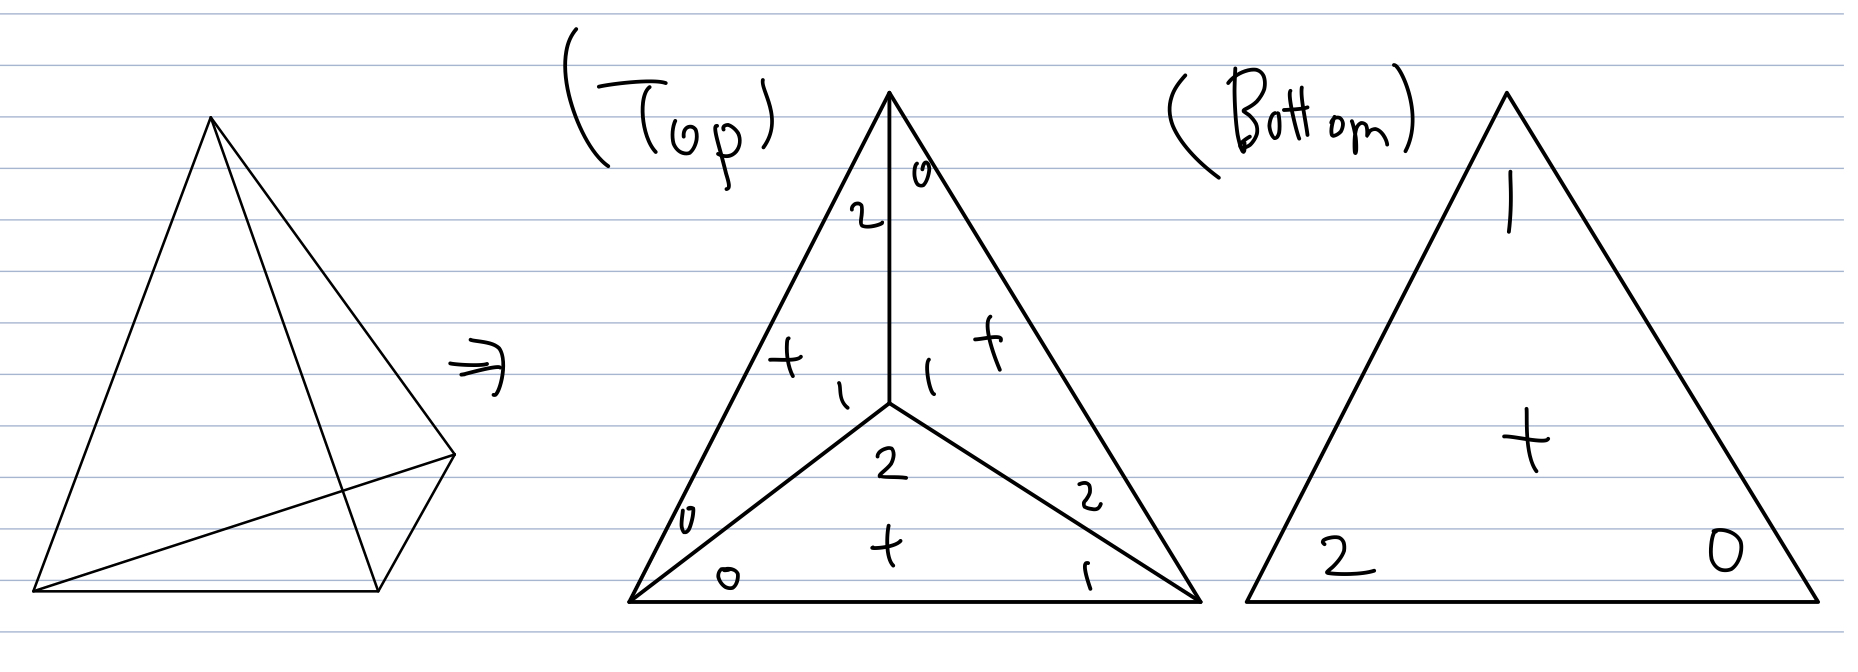
\includegraphics[width=.5\linewidth]{img/orientation_tetrahedron.jpeg}
    \caption{Orientation of a tetrahedron}
    \label{fig:orientation_tetrahedron}
  \end{figure}
\end{exmp}

\begin{defn}
  Let $M$ be an $n$-dimensional orientable manifold.
  Choose $\sigma_i \in C_n(M)$ and signs $\sgn_i \in \{ -1, 1 \}$ such that $M = \sigma_1 \cup \cdots \cup \sigma_k$ and $\sum \sgn_i \partial \sigma_i = 0$.
  The class represented by $\sum \sgn_i \sigma_i \in \ker(\partial)$ in $H_n(M)$ is called a fundamental class $[M]$.
\end{defn}

\begin{thm}\label{fundamental_class_generator}
  If $M$ connected, then $[M]$ is a generator of $H_n(M)$.
\end{thm}

\begin{proof}
  By Poincare Duality(which will be discussed later (\ref{poincare_duality_1})), $H_n(M) \cong H^0(M) = \mathbb{Z}$.
  Let $\sum c_i \sigma_i$ represent a generator of $H_n(M)$ where $c_i \in \mathbb{Z}$.
  Then $\sum \sgn_i \sigma_i = \lambda\sum c_i \sigma_i = \sum (\lambda c_i) \sigma_i$ for some $\lambda \in \mathbb{Z}$.
  Since each $\lambda c_i = \sgn_i \in \{ -1, 1 \}$, $\lambda$ must be 1 or -1.
  Therefore, the class represented by $\sum \sgn_i \sigma_i$ is a generator of $H_n(M)$.
\end{proof}

\begin{cor}
  There are two fundamental classes for any connected orientable manifold.
\end{cor}

\begin{proof}
  By (\ref{fundamental_class_generator}), a fundamental class $[M]$ is a generator of $H_n(M) = \mathbb{Z}$.
  Since $\mathbb{Z}$ has exactly two generators $1, -1$, $M$ has exactly two fundamental classes.
\end{proof}

\begin{defn}
  Let $M$ be a connected, orientable manifold.
  Then a choice of a fundamental class is called an orientation of $M$.
\end{defn}

\subsection{Poincare Duality(Version 1)}

\begin{thm}\label{poincare_duality_1}
  If $M$ is an orientable closed $n$-manifold, then
  \begin{align*}
    H^k(M; G) \cong H_{n - k}(M; G)
  \end{align*}
  for any integer $0 \leq k \leq n$ and an abelian group $G$.
\end{thm}

\begin{rem}
  If $M$ is not orientable, Poincare Duality holds when $G = \mathbb{Z} / 2$.
  In other words,
  \begin{align*}
    H^k(M; \mathbb{Z} / 2) \cong H_{n - k}(M; \mathbb{Z} / 2).
  \end{align*}
  For instance,
  \begin{center}
    \begin{tabular}{| l | l | l | l |} \hline
      $H_{\ast}(\RP^2; \mathbb{Z})$ & 0                & $\mathbb{Z} / 2$ & $\mathbb{Z}$ \\ \hline
      $H^{\ast}(\RP^2; \mathbb{Z})$ & $\mathbb{Z} / 2$ & 0                & $\mathbb{Z}$ \\ \hline
    \end{tabular}
  \end{center}
  so Poincare Duality does not hold in this case.
  However, with $\mathbb{Z} / 2$,
  \begin{center}
    \begin{tabular}{| l | l | l | l |} \hline
      $H_{\ast}(\RP^2; \mathbb{Z} / 2)$ & $\mathbb{Z} / 2$ & $\mathbb{Z} / 2$ & $\mathbb{Z} / 2$ \\ \hline
      $H^{\ast}(\RP^2; \mathbb{Z} / 2)$ & $\mathbb{Z} / 2$ & $\mathbb{Z} / 2$ & $\mathbb{Z} / 2$ \\ \hline
    \end{tabular}
  \end{center}
  so Poincare Duality holds in this case.
\end{rem}

\begin{defn}
  The $k$th Betti number of a manifold $M$ is defined to be $b_k = \rank(H^k(M; \mathbb{Z}))$.
\end{defn}

\begin{thm}
  $b_k = b_{n - k}$ for all $k$ if $M$ is a closed orientable $n$-manifold.
\end{thm}

\begin{proof}
  By the Universal Coefficient Theorem, $\rank(H^k(M)) = \rank(H_k(M))$.
  By Poincare Duality, $\rank(H^k(M)) = \rank(H_{n - k}(M))$.
  Therefore, $b_k = \rank(H^k(M)) = \rank(H_{n - k}(M)) = \rank(H^{n - k}(M)) = b_{n - k}$.
\end{proof}

\subsection{Cap Products}
There is a nice way to explicitly write down the isomorphism when $G$ is a commutative ring.

\begin{defn}
  Let a space $X$ and a commutative ring $R$ be given.
  For any $k \geq l$, define the cap product
  \begin{center}
    \begin{tikzcd}[cells={nodes={minimum height=2em}}]
      \frown: & C_k(X; R) \otimes C^l(X; R) \arrow[r] & C_{k - l}(X; R) \\
              & \sigma \otimes \phi \arrow[r, maps to]         & \phi(\sigma\vert_{[v_0,\cdots,v_l]})\sigma\vert_{[v_l, \cdots, v_k]}
    \end{tikzcd}
  \end{center}
\end{defn}

\begin{thm}\label{cap_product_formula}
  $\partial (\sigma \frown \phi) = (-1)^l((\partial \sigma) \frown \phi - \sigma \frown (\partial \phi))$.
\end{thm}

\begin{proof}
  Let $k \geq l, \sigma \in C_{k + 1}(X; R), \phi \in C^l(X; R)$ be given.
  \begin{align*}
    (\partial \sigma) \frown \phi
      &= (\sum_{j} (-1)^j \sigma\vert_{[v_0, \cdots, \hat{v}_j, \cdots, v_k]}) \frown \phi \\
      &= \sum_{j} (-1)^j (\sigma\vert_{[v_0, \cdots, \hat{v}_j, \cdots, v_k]} \frown \phi) \\
      &= \sum_{j = 1}^l (-1)^j \phi(\sigma\vert_{[v_0, \cdots, \hat{v}_j, \cdots, v_{l + 1}]})\sigma\vert_{[v_{l + 1}, \cdots, v_k]}
         + \sum_{j = l + 1}^{k} (-1)^j \phi(\sigma\vert_{[v_0, \cdots, v_{l}]})\sigma\vert_{[v_l, \cdots, \hat{v}_j, \cdots, v_k]} \\
      &= \sum_{j = 1}^l (-1)^j \phi(\sigma\vert_{[v_0, \cdots, \hat{v}_j, \cdots, v_{l + 1}]})\sigma\vert_{[v_{l + 1}, \cdots, v_k]} 
         + (-1)^{l + 1}\phi(\sigma\vert_{[v_0, \cdots, v_l, \hat{v}_{l + 1}]})\sigma\vert_{[v_{l + 1}, \cdots, v_k]} \\
      &+ (-1)^{l}\phi(\sigma\vert_{[v_0, \cdots, v_l]})\sigma\vert_{[\hat{v}_l, v_{l + 1}, \cdots, v_k]}
         + \sum_{j = l + 1}^{k} (-1)^j \phi(\sigma\vert_{[v_0, \cdots, v_{l}]})\sigma\vert_{[v_l, \cdots, \hat{v}_j, \cdots, v_k]} \\
      &= \sum_{j = 1}^{l + 1} (-1)^j \phi(\sigma\vert_{[v_0, \cdots, \hat{v}_j, \cdots, v_{l + 1}]})\sigma\vert_{[v_{l + 1}, \cdots, v_k]} 
         + \sum_{j = l}^{k} (-1)^j \phi(\sigma\vert_{[v_0, \cdots, v_{l}]})\sigma\vert_{[v_l, \cdots, \hat{v}_j, \cdots, v_k]}.
  \end{align*}
  We will compute each summand.
  \begin{align*}
    \sum_{j = 1}^{l + 1} (-1)^j \phi(\sigma\vert_{[v_0, \cdots, \hat{v}_j, \cdots, v_{l + 1}]})\sigma\vert_{[v_{l + 1}, \cdots, v_k]} 
      &= \phi(\sum_{j = 1}^{l + 1} (-1)^j \sigma\vert_{[v_0, \cdots, \hat{v}_j, \cdots, v_{l + 1}]})\sigma\vert_{[v_{l + 1}, \cdots, v_k]} \\
      &= \phi(\partial \sigma\vert_{[v_0, \cdots, v_{l + 1}]})\sigma\vert_{[v_{l + 1}, \cdots, v_k]} \\
      &= \sigma \frown \delta\phi.
  \end{align*}
  On the other hand,
  \begin{align*}
    \sum_{j = l}^{k} (-1)^j \phi(\sigma\vert_{[v_0, \cdots, v_{l}]})\sigma\vert_{[v_l, \cdots, \hat{v}_j, \cdots, v_k]}
      &= (-1)^l \sum_{j = 0}^{k - l} (-1)^j \phi(\sigma\vert_{[v_0, \cdots, v_{l + j}]})\sigma\vert_{[v_l, \cdots, \hat{v}_{l + j}, \cdots, v_k]} \\
      &= (-1)^l \partial(\phi(\sigma\vert_{[v_0, \cdots, v_{l + j}]})\sigma\vert_{[v_l, \cdots, v_k]}) \\
      &= (-1)^l \partial(\sigma \frown \phi).
  \end{align*}
  Therefore, we obtain the desired result $\partial (\sigma \frown \phi) = (-1)^l((\partial \sigma) \frown \phi - \sigma \frown (\delta \phi))$.
\end{proof}

\begin{thm}
  $\frown: C_k(X; R) \otimes C^l(X; R) \rightarrow C_{k - l}(X; R)$ induces a map $H_k(X; R) \otimes H^l(X; R) \rightarrow H_{k - l}(X; R)$.
\end{thm}

\begin{proof}
  Let $[\sigma] \in H_k(X; R)$ and $[\phi] \in H^l(X; R)$ be given where $\sigma \in C_k(X; R)$ and $\phi \in C^l(X; R)$.
  Then $\partial(\sigma) = \delta(\phi) = 0$.
  By (\ref{cap_product_formula}), $\partial(\sigma \frown \phi) = (-1)^l(0 - 0) = 0$.
  Therefore, $\sigma \frown \phi$ represents a class in $H_{k - l}(X; R)$.
\end{proof}

\subsection{Poincare Duality(Version 2)}

\begin{thm}\label{poincare_duality_2}
  If $M$ is an orientable closed $n$-manifold, let $[M] \in H_n(M)$ be a fundamental class for $M$, and let $R$ be a commutative ring.
  View $[M] \in H_n(M; R)$.
  Then the map
  \begin{center}
    \begin{tikzcd}[cells={nodes={minimum height=2em}}]
      H^l(M; R) \arrow[r] & H_{n - l}(M; R) \\
      \phi \arrow[r, maps to] & \left[M\right] \frown \phi
    \end{tikzcd}
  \end{center}
  is an $R$-module isomorphism.

  If $M$ is not orientable, then $[M] \in H_n(M; \mathbb{Z} / 2)$ still exists, and we have
  \begin{center}
    \begin{tikzcd}[cells={nodes={minimum height=2em}}]
      H^l(M; \mathbb{Z} / 2) \arrow[r] & H_{n - l}(M; \mathbb{Z} / 2) \\
      \phi \arrow[r, maps to] & \left[M\right] \frown \phi
    \end{tikzcd}
  \end{center}
\end{thm}

\subsection{Differential Forms on $\mathbb{R}^n$}

\begin{defn}
  Let $dx_1, \cdots, dx_n$ be formal indeterminates.
  Let $V$ be the vector space over $\mathbb{R}$ generated by $dx_1, \cdots, dx_n$.
  Let $\Omega^{\ast}$ be the $\mathbb{R}$-algebra generated by $dx_1, \cdots, dx_n$ module relations $dx_i \wedge dx_i = 0$ and $dx_i \wedge dx_j = - dx_j \wedge dx_i$.
\end{defn}

\begin{lem}
  The dimension of $\Omega^{\ast}$ over $\mathbb{R}$ is $2^n$.
\end{lem}

\begin{proof}
  $\Omega^{\ast}$ is generated by the set of elements of the form $dx_{i_1} \wedge \cdots \wedge dx_{i_k}$ where $0 \leq k \leq n$ and $i_1 < \cdots < i_k$.
  This is because of the two relations of $\Omega^{\ast}$.
  We denote it by $dx_{I}$ where $I = \{ i_1, \cdots, i_k \}$.
  Then there are exactly $2^n$ $I$'s, so the dimension is $2^n$.
\end{proof}

\begin{defn}
  Let $U \subset \mathbb{R}^n$ be open.
  Then $\Omega^{\ast}(U) = C^{\infty}(U) \otimes \Omega^{\ast}$.
\end{defn}

\begin{lem}
  $\Omega^{\ast}(U)$ is a graded, sign-commutative $\mathbb{R}$-algebra.
\end{lem}

\begin{proof}
  $\Omega^{\ast}(U)$ is a vector space over $\mathbb{R}$ because addition can be defined in a trivial way and for any $c \in \mathbb{R}$ and $f \otimes dx_I \in \Omega^{\ast}(U)$, $c(f \otimes dx_I) = (cf) \otimes dx_I$.
  Moreover, $(f_Idx_I) \wedge (f_Jdx_J) = (f_If_J)(dx_I \wedge dx_J)$ is a well-defined multiplication.
  It is easy to see that the multiplication, addition and scalar multiplication commute.
  Thus $\Omega^{\ast}(U)$ is a $\mathbb{R}$-algebra.
  Moreover, $\Omega^{\ast}(U) = \oplus_{k=1}^{n} \Omega^k(U)$ where $\Omega^k(U) = \{ \sum_{\abs{I} = k} f_Idx_I \}$.
  Finally, for any $\omega_1 \in \Omega^{k_1}(U), \omega_2 \in \Omega^{k_2}(U), \omega_1 \wedge \omega_2 = (-1)^{k_1k_2} \omega_2 \wedge \omega_1$.
\end{proof}
\end{document}
